\part{Progress on the GAN}
\label{part:progress_on_gan}


%------------------------------------
\section{A short reminder what this project is about}
\label{sec:short_reminder}

As the title suggests this project is all about car design.
The goal is to create and have control over a generative adversarial network (GAN) capable of generating pleasing images of cars that don't exist.
The control over this GAN is the most crucial part of this project.
Not only will having control over the GAN allow for exploring similar car designs, but it will also validate the system is not just generative. 


%------------------------------------
\section{The choice for a pretrained GAN}
\label{sec:pretraind_gan}

In earlier assignments, it was discussed that the required training data for the GAN, images of cars, could be scraped from the web.
Thus a custom scraper could be written to collect images.
It was advised for this scraper to work by using popular car auction websites as its source since these would allow for collecting meta-data as well.
However, training a GAN is a computationally hard task.
For example, training a StyleGAN2 model would take weeks, if not months, on the most powerful system available for this project.

Luckily StyleGAN offers a wide range of pre-trained networks \citep{stylegan2}.
Multiple pre-trained models for StyleGAN on the car-related LSUN dataset are available for download by NVIDIA, creator of StyleGAN2 \citep{stylegan2}.
This LSUN dataset is the same one that is part of the LSUN-Stanford Car dataset by \citet{cardb} already heavily discussed in previous assignments.
Since this dataset was considered as a training dataset if the scraping wouldn't work and the computation power needed to train a GAN is just not available for this project, the choice for opting for such a pre-trained model seemed logical.
This was discussed and accepted by both Professor Wiggins as well as Mr Harley.

It was opted to go for the 'config f' variant of the LSUN car database pre-trained StyleGAN2 model.
This was done since this configuration offers the highest resolution possible, 512x512, and produces not only very pleasing but also interesting results.
Some images generated by the GAN for this project are given in figure \ref{fig:straightexports}.

\begin{figure*}
\centering
\begin{subfigure}{.3\textwidth}
  \centering
  \includegraphics[width=\textwidth]{images/Attempt at reflection.png}
  \caption{Sports convertible}
  \label{fig:reflection}
\end{subfigure}%
\hspace{.02\textwidth}
\begin{subfigure}{.3\textwidth}
  \centering
  \includegraphics[width=\textwidth]{images/Challenging angle (4).png}
  \caption{Double front car}
  \label{fig:doublefront}
\end{subfigure}
\hspace{.02\textwidth}
\begin{subfigure}{.3\textwidth}
  \centering
  \includegraphics[width=\textwidth]{images/Multi inspired car.png}
  \caption{Multi model inspired design}
  \label{fig:multiinspired}
\end{subfigure}
\captionsetup{width=.85\linewidth}
\caption{Multiple images generated by the used GAN for this project, settings and more info available on the GitHub repository for this project \citep{github_project}.}
\label{fig:straightexports}
\end{figure*}

%------------------------------------
\section{Extending the GANSpace tool}
\label{sec:ganspace_extended}

Since the settled on pre-trained GAN is working as intended, it was also already made to work with the GANSpace tool discussed in the previous assignments \citep{ganspace}.
For this, an extended version of the GANSpace tool was made.
This extended version has a new parameter to specify the used mode should be the one custom made for this project.
Besides this, some features were added to the tool as well, such as an option to export the current canvas, even if it has multiple images on it, all through an easy to use UI.

The extended GANSpace tool works flawlessly once installed, but installation is not as straight forward as it could be.
Since the tool is still relatively unknown and new with available setup instructions missing vital instructions, a more in-depth guide was made available on the GitHub repository for this project \citep{github_project}.
This guide makes use of a fresh install of Ubuntu 20.04 and a system with an NVIDIA GTX970.
Many scripts for and modifications to the GANSpace tool are made to make reproducibility easier.
All of the missing steps not discussed in the original GitHub repository of the GANSpace tool \citep{ganspace_git}, are listed in the thorough documentation of this project's GitHub \citep{github_project}. 


\begin{figure*}
\begin{subfigure}{.45\textwidth}
  \centering
  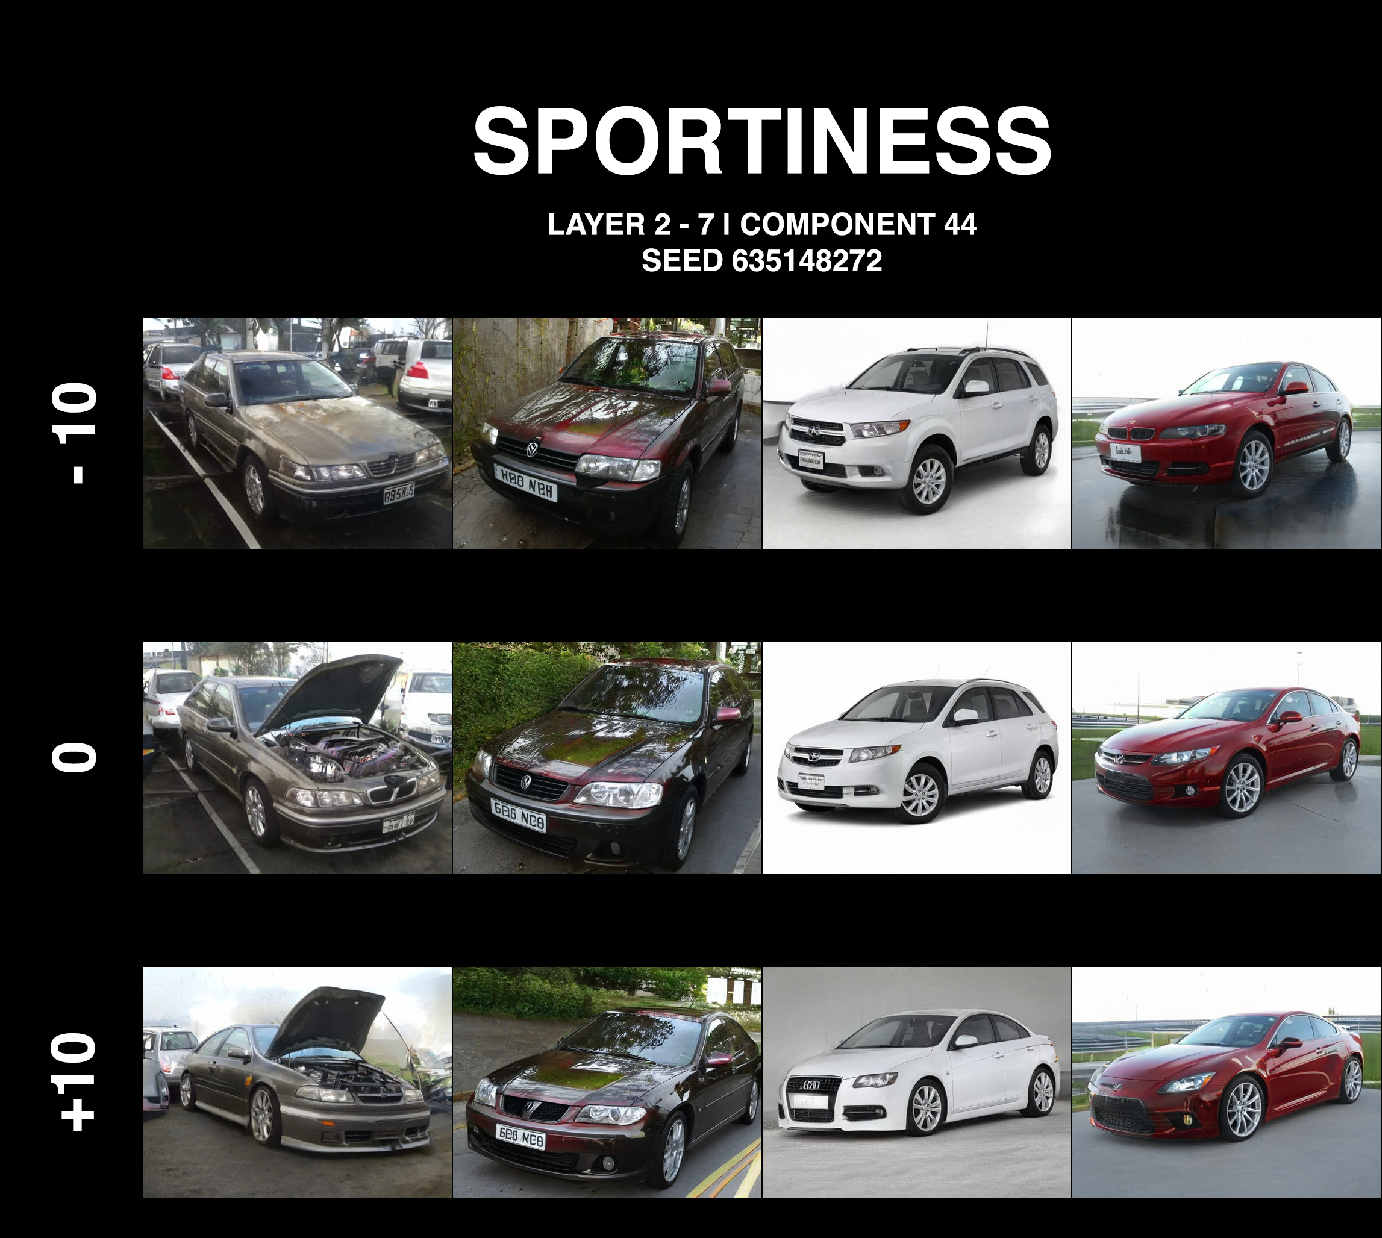
\includegraphics[width=\textwidth]{images/Sportiness.pdf}
  \caption{Component found to influence sportiness of the generated cars.}
  \label{fig:sportiness}
\end{subfigure}%
\hspace{.04\textwidth}
\begin{subfigure}{.45\textwidth}
  \centering
  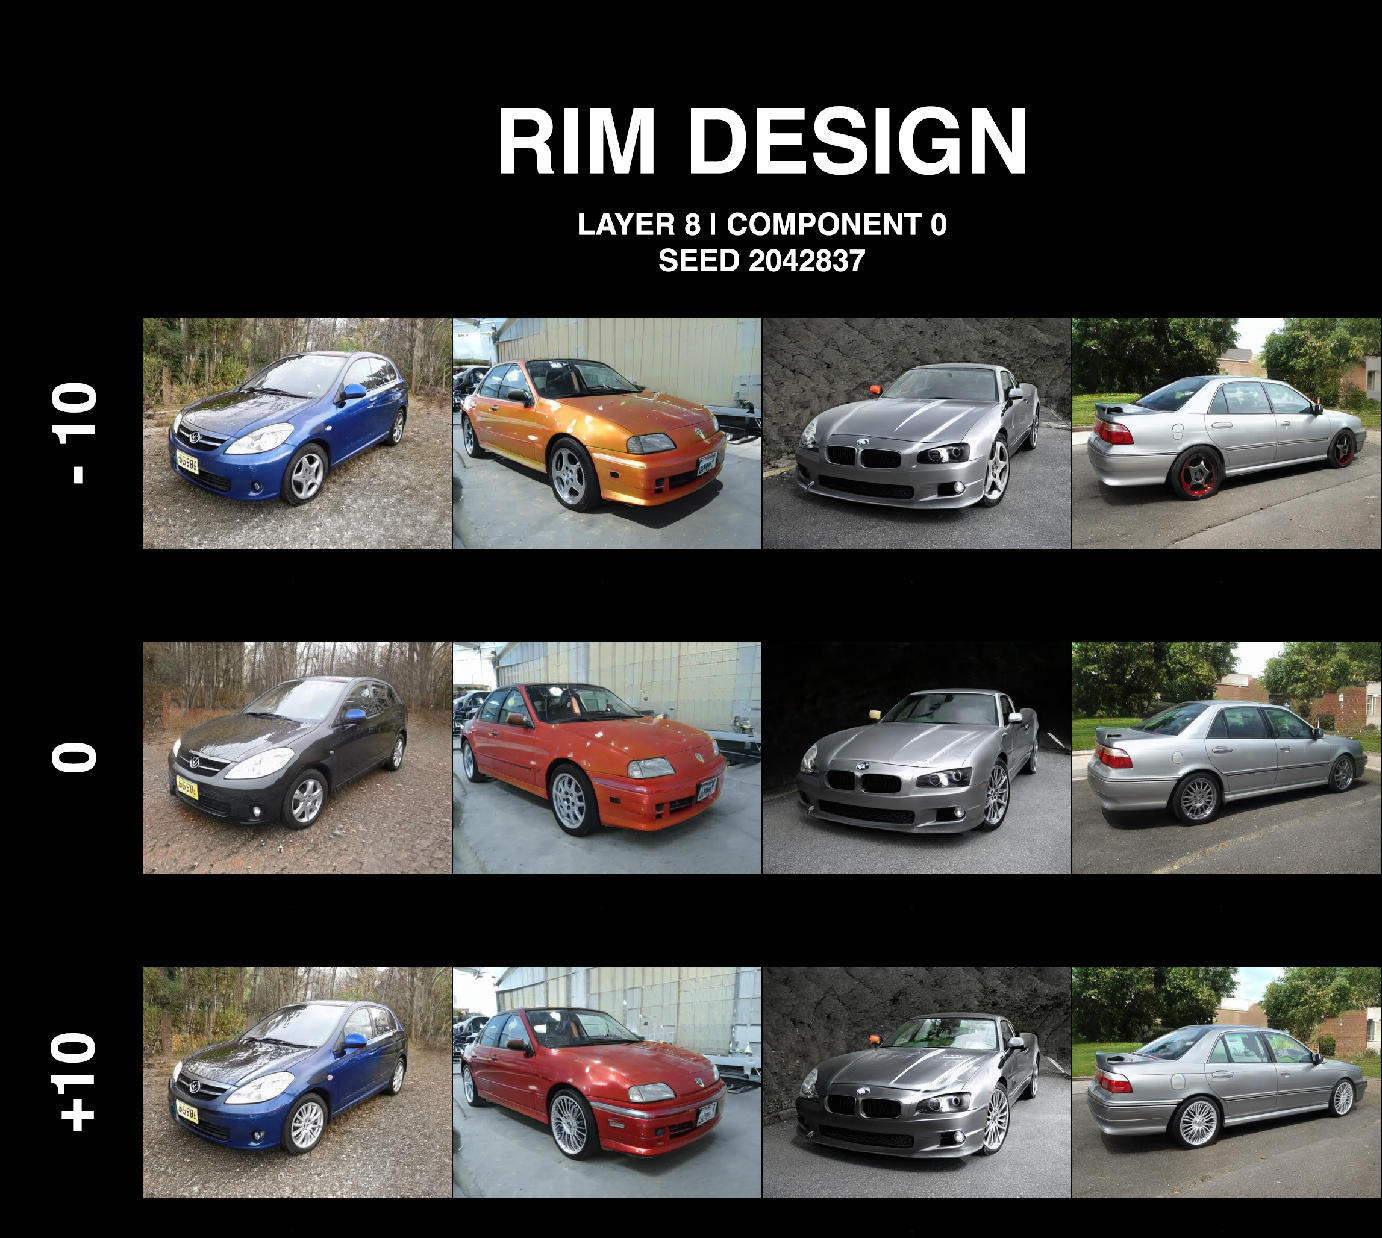
\includegraphics[width=\textwidth]{images/rim_design.pdf}
  \caption{Component found to influence the rim design of the generated cars in a pretty standalone fashion.}
  \label{fig:rimdesign}
\end{subfigure}
\centering
\captionsetup{width=.85\linewidth}
\caption{Baseline images, labeled '0', from the GAN and variants by manipulating interesting found components using the extended GANSpace tool. Settings and more info available on this project's GitHub repository \citep{github_project}.}
\label{fig:ganspaceexports}
\end{figure*}